\begin{center}

  \begin{tabular}{rp{16cm}lp{20cm}}%{rl}

  % after \\: \hline or \cline{col1-col2} \cline{col3-col4} ...

  论文地址:& \href{https://arxiv.org/pdf/2010.13993.pdf}{https://arxiv.org/pdf/2010.13993.pdf} \\
  来源:& ICLR, 2021\\
  作者:& Qian Huangz, Horace He, et al. \\

  源码:& \href{https://github.com/CUAI/CorrectAndSmooth}{CorrectAndSmooth} \\

%  slides:& \href{http://yunshengb.com/wp-content/uploads/2017/03/nips_2018_r2l_workshop_talk.pdf}{{\footnotesize Convolutional Set Matching for Graph Similarity}}\\

  关键词:& \textbf{Label Propagation, Transductive node classification } \\

  写于:& \date{2021-03-25}

  \end{tabular}

\end{center}

该论文\cite{huang2020combining}针对GNN的解释性不足,GNN模型越来越大的问题,提出了“小米加步枪” --- 用简单模型得到和GNN一样的水平。针对trnasductive的节点分类问题,作者使用浅层模型加上LP(Label Propagation)和两个后处理方法 --- Correct \& Smooth,达到或超过了GNN在一些transductive结点分类上的效果。

\paragraph{问题定义}
给定一个图$G = (V, E)$,结点特征矩阵为$X \in \mathbb{R}^{n \times p}$,结点集$V$可以分为$U, L$分别表示无标签、有标签结点子集。标签矩阵为$Y \in \mathbb{R}^{n \times c}$。目标就是基于以上所给的信息,预测$U$中结点的标签。

\paragraph{Correct and Smooth}
论文的方法总体过程可以分为三步:
\begin{enumerate}
	\item 使用浅层模型,在$L$上,根据结点的特征做一个基础的预测,即找到$\mathop{\arg\min}\limits_{f}\: l(f(x_i), y_i)$,得到基础预测$Z \in \mathbb{R}^{n\times c}$;
	\item 利用标签数据的信息去改正基础预测$Z$;
	\item 根据相邻结点的相似性,对改正后的预测进行平滑;
\end{enumerate}

\begin{figure}[h]
	\centering
	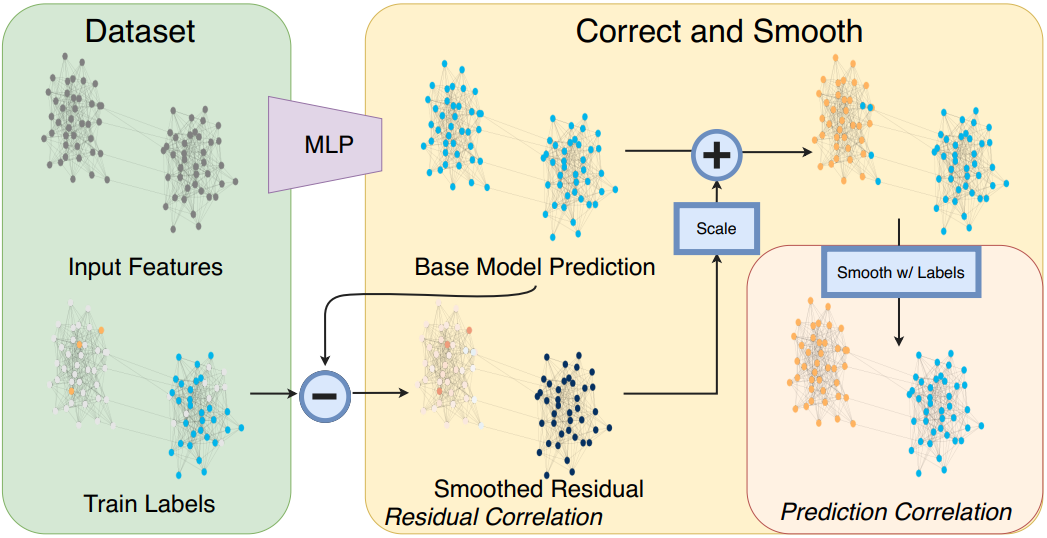
\includegraphics[width=.8\textwidth]{pics/C&S.png}
	\caption{Correct and Smooth}
	\label{fig:C&S}
\end{figure}

\subparagraph{Simple Base Predictor}
找到一个浅层模型$f$,如线性模型、MLP等,在训练数据($L$的子集)上达到最小经验损失。这一步并不会使用到图的结构,可以避免GNN模型的可扩展性问题。

\subparagraph{Correct error in base prediction with Residual Propagation}
在上一步已经有了一个基础的预测$Z$,而且有标签矩阵$Y$,可以根据二者在训练集($L_t$)上构建误差矩阵$E$,也就是residual,即:
$$
E_{L_t} = Z_{L_t} - Y_{L_t},\quad E_{L_v} = 0,\quad E_{U} = 0
$$
作者使用LP对$E$进行了平滑,平滑的公式为:
$$
\hat{E}=\underset{W \in \mathbb{R}^{n \times c}}{\arg \min } \operatorname{trace}\left(W^{T}(I-S) W\right)+\mu\|W-E\|_{F}^{2}
$$
其中$S$为$D^{-\frac{1}{2}}AD^{-\frac{1}{2}}$。上式的第一项保证$E$在$G$上的平滑,第二项保证$\hat{E}$不会偏离$E$太多。上式可以通过迭代求解,迭代式为:$E^{(t+1)} = (1-\alpha)E + \alpha SE^{(t)}$,其中$\alpha = \frac{1}{1+\mu},\: E^{(0)} = E$。得到了$\hat{E}$然后呢?当然是修正$Z$啦!$Z^{(r)} = Z + \hat{E}$。

那么问题来了,为什么要这样呢?\tbc{red}{$Z$中的误差会沿着图中的边传播,结点$i$处的误差会使得$i$的邻居产生类似的误差,应当将这种误差 --- 不确定性传播出去,即文中的error-correlation}! 

但是有一个问题:
$$
\left\|E^{(t+1)}\right\|_{2} \leq(1-\alpha)\|E\|+\alpha\|S\|_{2}\left\|E^{(t)}\right\|_{2}=(1-\alpha)\|E\|_{2}+\alpha\left\|E^{(t)}\right\|_{2}
$$
因此$\left\|E^{(t)}\right\|_{2} \leq\|E\|_{2}$,可见在迭代求解过程中误差信息有一定损失,因此作者提出了对误差信息进行缩放。作者提出了两种缩放方法:
\begin{itemize}
	\item Autoscale。因为在$L_t$上的误差是知道的,因此以$L_t$上的平均误差为比例进行缩放。即$Z_{i,:}^{(r)}=Z_{i,:}+\sigma \hat{E}_{:, i} /\left\|\hat{E}_{:, i}^{T}\right\|_{1} for\:i \in U$,其中$\sigma = \frac{1}{|L_t|}\sum_{j \in L_t} ||e_j||_1$,其中$e_j$为$E$的$j-th$行;
	 
	\item Scaled Fixed Diffusion。在迭代过程中保持标签数据上的误差不变,即$E_U^{(t+1)} = [D^{-1}AE^{(t)}]_U,\: E_L^{(t)} = E_L$;
\end{itemize}


\subparagraph{Smoothing final prediction with Prediction Correlation}
通过上一步已经得到了$Z^{(r)}$,这一步是对$Z^{(r)}$的“平滑”。这一步的动机是:\textbf{相邻的结点相似,更可能具有相同的标签,即文中的prediction correlation},这一步再次借助LP对结点的标签分布进行平滑。

首先构造一个$G$中结点的标签分布$P \in \mathbb{R}^{n \times c}$,$P_{L_t} = Y_{L_t},\: G_{L_v, U} = Z^{(r)}_{L_v, U}$。接着就是平滑了,也就是一个迭代的过程:$P^{(t+1)} = (1-\alpha)P + \alpha SP^{(t)}$,一直迭代到收敛得到最终的收敛$\hat{Y}_{ij}$。

\paragraph{总结}

\begin{itemize}

	\item 没用一股脑地上深度模型(当然,GNN大多不是深层的)。浅层模型+LP在transductive node classification上的效果直追/超过了一些GNN模型;
	\item 论文中的方法效果不错,且大大降低了模型的参数量、学习时间,速度快;
	\item 不足的是只能进行transductive的任务,目前的趋势是inductive learning;
	\item 不知道该论文的方法在其他任务上会有怎样的效果;

\end{itemize}

